% =====================================================================
%  Lumen Spirits - Relazione progetto Tecnologie Web
%  Universita degli Studi di Padova - A.A. 2025/2026
%
%  Compilazione:
%    pdflatex lumen-spirits.tex
%    pdflatex lumen-spirits.tex   (seconda passata per indice)
% =====================================================================

\documentclass[11pt,a4paper]{article}

% ---- Encoding e lingua ----
\usepackage[utf8]{inputenc}
\usepackage[T1]{fontenc}
\usepackage[italian]{babel}
\usepackage{lmodern}

% ---- Layout pagina ----
\usepackage[a4paper,top=2.5cm,bottom=2.5cm,left=2.5cm,right=2.5cm,headheight=14pt]{geometry}
\usepackage{setspace}
\setstretch{1.15}

% ---- Pacchetti utili ----
\usepackage{graphicx}
\usepackage{xcolor}
\usepackage{booktabs}
\usepackage{array}
\usepackage{tabularx}
\usepackage{colortbl}
\usepackage{enumitem}
\usepackage{titlesec}
\usepackage{fancyhdr}
\usepackage{parskip}
\usepackage{ragged2e}

% ---- Hyperref (link colorati come nel PDF originale) ----
\usepackage[hidelinks]{hyperref}
\hypersetup{
  colorlinks=true,
  linkcolor=linkblue,
  urlcolor=linkblue,
  citecolor=linkblue,
  pdftitle={Lumen Spirits - Relazione progetto Tecnologie Web},
  pdfauthor={Gruppo Lumen Spirits},
}

% ---- Palette ----
\definecolor{linkblue}{HTML}{1F4E96}
\definecolor{tableheader}{HTML}{A8C6D0}   % azzurrino intestazioni tabelle
\definecolor{tablerule}{HTML}{4A4A4A}
\definecolor{lightgray}{HTML}{888888}
\definecolor{unipdred}{HTML}{9B0014}

% ---- Stile heading (numerati come nel PDF originale) ----
\titleformat{\section}{\Huge\bfseries}{\thesection.}{0.5em}{}
\titleformat{\subsection}{\LARGE\bfseries}{\thesubsection}{0.5em}{}
\titleformat{\subsubsection}{\Large\bfseries}{\thesubsubsection}{0.5em}{}
\newcommand{\subsubsubsection}[1]{\paragraph{#1}\mbox{}\\}

\titlespacing*{\section}{0pt}{1.5em}{0.8em}
\titlespacing*{\subsection}{0pt}{1.2em}{0.5em}
\titlespacing*{\subsubsection}{0pt}{1em}{0.4em}

% ---- Header/footer di pagina (titolo a sinistra, numero a destra) ----
\pagestyle{fancy}
\fancyhf{}
\fancyhead[L]{\small Lumen Spirits -- E-commerce di lampade riciclate}
\fancyfoot[C]{\thepage}
\renewcommand{\headrulewidth}{0pt}
\renewcommand{\footrulewidth}{0pt}

% ---- Liste puntate piu compatte ----
\setlist[itemize]{leftmargin=1.5em,itemsep=0.2em,topsep=0.3em}
\setlist[itemize,2]{leftmargin=1.5em,label=$\circ$}

% ---- Comando per la riga orizzontale di separazione tra sezioni ----
\newcommand{\sectionrule}{\vspace{0.5em}\noindent\rule{\linewidth}{0.4pt}\vspace{0.5em}}

% =====================================================================
\begin{document}

% =====================================================================
% Frontespizio
% =====================================================================
\begin{titlepage}
  \thispagestyle{empty}
  \centering

  \vspace*{1cm}

  % TODO: aggiungere logo UniPD in img/logo-unipd.png
  
\includegraphics[width=0.35\textwidth]{img/logo_unipd.png}\\[0.5cm]
  % \fbox{\parbox{0.45\textwidth}{\centering\vspace{1.5cm}\textit{[ Logo UniPD -- img/logo-unipd.png ]}\vspace{1.5cm}}}\\[1cm]

  {\Huge\bfseries Lumen Spirits}\\[0.4cm]
  {\Large E-commerce di lampade artigianali da bottiglie riciclate}\\[0.2cm]
  {\large Relazione progetto di Tecnologie Web}\\[0.1cm]
  {\large Anno accademico 2025/2026}\\[1.5cm]

  % ---- Tabella componenti gruppo ----
  {\large\bfseries Componenti del Gruppo}\\[0.3cm]
  \begin{tabular}{|p{5cm}|p{3cm}|}
    \hline
    % TODO: sostituire con nomi e matricole reali
    Davide Facco & \textit{matricola} \\
    \hline
    Membro 2 & \textit{matricola} \\
    \hline
    Membro 3 & \textit{matricola} \\
    \hline
    Membro 4 & \textit{matricola} \\
    \hline
  \end{tabular}\\[1.2cm]

  % ---- Tabella informazioni sito ----
  {\large\bfseries Informazioni sul sito}\\[0.3cm]
  \begin{tabular}{|>{\columncolor{tableheader}}p{4.5cm}|p{8cm}|}
    \hline
    Login consegna & \textit{login\_consegna} \\
    \hline
    Link sito web & \textit{http://tecweb.studenti.math.unipd.it/.../index.html} \\
    \hline
    Email referente gruppo & \textit{referente@studenti.unipd.it} \\
    \hline
  \end{tabular}\\[1.2cm]

  % ---- Tabella credenziali accesso ----
  {\large\bfseries Credenziali di accesso}\\[0.3cm]
  \begin{tabular}{|p{3cm}|p{3cm}|p{3cm}|}
    \hline
    \rowcolor{tableheader}
    \textbf{Ruolo} & \textbf{Username} & \textbf{Password} \\
    \hline
    Admin & admin & admin \\
    \hline
    User & user & user \\
    \hline
  \end{tabular}

  \vfill
\end{titlepage}

% =====================================================================
% Sommario
% =====================================================================
\newpage
\pagenumbering{arabic}
\setcounter{page}{1}

{\Huge\bfseries Sommario}\\[1em]
\renewcommand{\contentsname}{}
\setcounter{tocdepth}{4}
\tableofcontents

\newpage

% =====================================================================
% 1. Abstract
% =====================================================================
\section{Abstract}

Il progetto ``Lumen Spirits'' si basa sulla creazione di una piattaforma e-commerce dedicata alla vendita di lampade artigianali realizzate a partire da bottiglie di vetro recuperate. Per noi il tema dell'\textbf{upcycling} e del consumo consapevole rappresenta un punto di partenza valoriale: con questo progetto intendiamo promuovere una maggiore sensibilit\`a verso il riuso creativo e il design sostenibile.

La piattaforma permette ai visitatori di sfogliare il catalogo, ricercare prodotti specifici, leggere schede dettagliate e aggiungere articoli al carrello senza barriere di registrazione. Gli utenti registrati possono completare l'acquisto, salvare un indirizzo di spedizione e consultare la cronologia dei propri ordini. Gli amministratori dispongono di un pannello dedicato per creare, modificare ed eliminare i prodotti del catalogo, gestire i ruoli degli utenti, monitorare gli ordini e gestire i messaggi ricevuti dal modulo contatti.

\sectionrule

% =====================================================================
% 2. Analisi del sito
% =====================================================================
\section{Analisi del sito}

\subsection{Target di riferimento}
Il sito ha una grafica ed un tono \textit{warm} e minimalista, pensati per avvicinare un pubblico attento al design e alla sostenibilit\`a ambientale. Allo stesso tempo costituisce una piattaforma universale: chiunque cerchi un oggetto di arredo unico o un regalo dal valore simbolico pu\`o trovare un'esperienza di navigazione semplice e accessibile. Sono stati inclusi ausili alla navigazione e accorgimenti volti a garantire l'accessibilit\`a del sito, in modo da non escludere nessuna categoria di utenti.

Di seguito alcune possibili ricerche sui motori di ricerca che gli utenti potrebbero fare:
\begin{itemize}
  \item Lumen Spirits
  \item Lampade da bottiglie riciclate
  \item Upcycled lamp
  \item Lampade artigianali Italia
  \item Decor sostenibile
  \item Idee regalo eco-friendly
  \item Illuminazione di design riciclata
  \item Acquisto lampade online
  \item Profilo Lumen Spirits
  \item Accedi Lumen Spirits.
\end{itemize}

La facilit\`a di reperimento delle informazioni \`e garantita anche quando l'utente ha solo una vaga idea di ci\`o che cerca: la barra di ricerca presente nel catalogo, basata su filtri dinamici lato client, consente di restringere la selezione in tempo reale e di raggiungere ``il tiro perfetto'' anche quando il termine inserito \`e parziale o approssimativo.

\subsubsection{Tipologie di utente}
Sono stati individuati due tipi di utente: l'utente amministratore (admin) e l'utente semplice (user).

\subsubsubsection{2.1.1.1\quad Admin}
Staff incaricato della gestione del catalogo e degli ordini.
\begin{itemize}
  \item ha accesso a tutti i prodotti e a tutti gli ordini registrati nel sistema;
  \item pu\`o creare nuovi prodotti, modificarne i dettagli o eliminarli;
  \item pu\`o promuovere altri utenti al ruolo di amministratore.
\end{itemize}

\subsubsubsection{2.1.1.2\quad User}
Pu\`o essere a sua volta:
\begin{itemize}
  \item \textbf{Visitatore}: utente che accede al sito senza effettuare alcun login o registrazione
  \begin{itemize}
    \item pu\`o sfogliare il catalogo, leggere le schede prodotto e usare la ricerca;
    \item pu\`o aggiungere articoli al carrello, memorizzato localmente nel browser.
  \end{itemize}
  \item \textbf{Utente registrato}: utente che accede al sito effettuando login o registrazione
  \begin{itemize}
    \item pu\`o effettuare tutte le azioni del visitatore;
    \item pu\`o completare il checkout, salvare i propri dati anagrafici e l'indirizzo di spedizione;
    \item pu\`o consultare lo storico degli ordini effettuati.
  \end{itemize}
\end{itemize}

\subsection{Funzionalit\`a sviluppate}
\begin{itemize}
  \item \textbf{Funzionalit\`a pubbliche} accessibili a qualsiasi tipo di utente:
  \begin{itemize}
    \item consultazione del catalogo con presentazione di ciascun prodotto, materiali utilizzati e descrizione artigianale;
    \item ricerca live con filtraggio immediato dei risultati;
    \item gestione di un carrello persistente nel browser anche senza autenticazione.
  \end{itemize}
  \item \textbf{Gestione account utente}:
  \begin{itemize}
    \item registrazione con username, email e password;
    \item modifica dei dati anagrafici e dell'indirizzo di spedizione in qualsiasi momento;
    \item cambio password.
  \end{itemize}
  \item \textbf{Checkout e ordini} (core business del sito):
  \begin{itemize}
    \item completamento dell'ordine tramite modulo riepilogativo con calcolo dinamico del totale;
    \item visualizzazione dello storico degli ordini effettuati nell'area profilo.
  \end{itemize}
  \item \textbf{Funzionalit\`a amministrative}:
  \begin{itemize}
    \item CRUD completo dei prodotti del catalogo;
    \item visualizzazione tabellare di tutti gli ordini per la pianificazione della logistica;
    \item gestione dei ruoli utente attraverso il flag \texttt{isAdmin}.
  \end{itemize}
  \item \textbf{Stampa}:
  \begin{itemize}
    \item l'utente pu\`o stampare le pagine del sito, in particolare la ricevuta d'ordine, grazie a un foglio di stile dedicato.
  \end{itemize}
\end{itemize}

\sectionrule

% =====================================================================
% 3. Struttura e Design del sito
% =====================================================================
\section{Struttura e Design del sito}

Prima di iniziare la fase di scrittura del codice abbiamo disegnato una bozza di come il sito sarebbe dovuto apparire a lavori finiti, creando cos\`i delle aspettative e dei metodi di paragone mediante i quali sarebbe stato poi possibile verificare durante e alla fine che il lavoro rappresentasse la visione iniziale del progetto.

Il design che abbiamo creato \`e ampio e poco profondo, raggiungendo un'ampiezza di 5 voci, definite dal menu di navigazione, ed una profondit\`a massima raggiungibile di 3.

Le 5 voci del menu sono, in ordine:
\begin{itemize}
  \item \textbf{Home}: pagina principale dove accogliamo l'utente con presentazione del progetto e prodotti in evidenza;
  \item \textbf{Catalogo}: griglia completa dei prodotti disponibili con filtri di ricerca e paginazione;
  \item \textbf{Carrello}: riepilogo degli articoli aggiunti con possibilit\`a di modificare quantit\`a o rimuovere voci;
  \item \textbf{Contatti}: informazioni sul gruppo, modulo per richieste, recapiti email e social;
  \item \textbf{Profilo}: dopo il login mostra dati dell'utente, indirizzo e storico ordini (per gli admin: pannello di gestione catalogo, utenti, ordini e messaggi ricevuti).
\end{itemize}

Le altre pagine che \`e possibile visualizzare sono:
\begin{itemize}
  \item \textbf{Login}: pagina che compare quando un utente seleziona l'icona del profilo nel men\`u senza aver ancora effettuato l'accesso. Permette di effettuare il login con username e password, o di recarsi alla pagina di registrazione;
  \item \textbf{Registrazione}: permette di creare un nuovo account inserendo username, email e password;
  \item \textbf{Scheda prodotto}: pagina dedicata al singolo articolo, con galleria immagini, descrizione estesa, prezzo e bottone per aggiungere al carrello;
  \item \textbf{Modifica prodotto}: pagina riservata agli amministratori per creare o aggiornare un articolo del catalogo;
  \item \textbf{Errore 404}: l'utente cerca una pagina sconosciuta;
  \item \textbf{Errore 500}: c'\`e un errore da parte del server.
\end{itemize}

\sectionrule

% =====================================================================
% 4. Progettazione
% =====================================================================
\section{Progettazione}

Successivamente alla fase di Design abbiamo iniziato a creare un progetto per costruire il sito. Questa fase ci \`e servita per avere una sorta di blueprint per capire come effettivamente i pezzi vadano uniti e per capire come farli funzionare insieme.

\subsection{Struttura del progetto}
Per creare la blueprint ci siamo forniti di un'applicazione esterna, \textbf{draw.io}, per disegnare la struttura ed avere dei riferimenti visivi:

\begin{center}
  % TODO: inserire diagramma blueprint in img/blueprint.png
  % 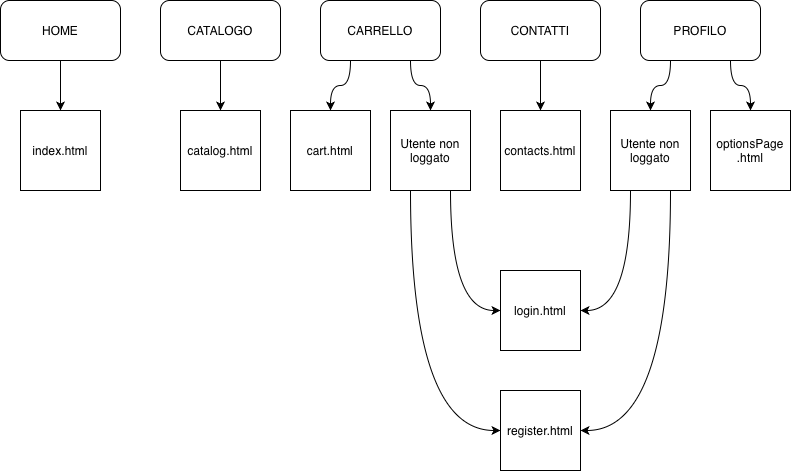
\includegraphics[width=0.85\textwidth]{img/blueprint.png}
  \fbox{\parbox{0.85\textwidth}{\centering\vspace{2cm}\textit{[ Diagramma blueprint draw.io -- placeholder ]}\\\small Home, Catalogo, Carrello, Contatti, Profilo con relative pagine dipendenti\vspace{2cm}}}
\end{center}

Abbiamo quindi disegnato tutte le pagine che volevamo fossero raggiungibili, dove i rettangoli con angoli arrotondati rappresentano le voci del menu, mentre i rettangoli rappresentano le pagine che effettivamente l'utente raggiunger\`a una volta cliccata la voce a seconda delle sue condizioni di visitatore o utente registrato.

\begin{center}
  % TODO: inserire diagramma flussi in img/flussi.png
  \fbox{\parbox{0.7\textwidth}{\centering\vspace{1.5cm}\textit{[ Diagramma flussi utente -- placeholder ]}\\\small Home $\to$ Catalogo $\to$ Scheda prodotto $\to$ Carrello $\to$ Checkout\vspace{1.5cm}}}
\end{center}

Abbiamo successivamente disegnato dei sentieri che un utente pu\`o fare dalla Home senza dover interagire con il menu, dove i cerchi sono delle azioni che l'utente deve fare per continuare il percorso. Abbiamo deciso di rendere raggiungibili \textbf{Catalogo} e \textbf{Carrello} direttamente dalla Home, poich\`e sono il cuore del sito e vogliamo riuscire a portare pi\`u utenti possibili al completamento dell'acquisto. Tutte le altre pagine rimangono raggiungibili in ogni momento attraverso il menu di navigazione.

\subsection{Strategia di sviluppo}
Come strategia di sviluppo abbiamo deciso di usare la tecnica \textbf{Mobile first}, dove si d\`a particolare attenzione agli utenti che accedono al sito dallo smartphone. Ogni pagina \`e stata inizialmente pensata per schermi pi\`u piccoli, dove la disposizione degli elementi informativi \`e risultata pi\`u complessa, per poi essere adattata e completata per schermi di dimensioni maggiori.

\subsection{Emotional Design e scelta dei colori}
Per quanto riguarda l'\textbf{Emotional Design}, abbiamo scelto un approccio orientato alla fiducia, all'artigianalit\`a e al senso di calore domestico, piuttosto che all'intrattenimento. Trattandosi di oggetti artigianali realizzati con materiali di recupero, abbiamo evitato meccaniche di gamification (come badge di esclusivit\`a o ricompense a sorpresa) che avrebbero rischiato di banalizzare il valore del singolo pezzo.

Abbiamo invece lavorato sulla componente estetica attraverso la scelta cromatica. Abbiamo optato per sfumature di \textit{terracotta} e \textit{crema} come colori primari per richiamare i materiali naturali (terra, sabbia, legno) e per trasmettere calore, manualit\`a e attenzione ambientale, allontanandoci da palette fredde o eccessivamente sature.

\subsection{Struttura delle pagine}
La struttura di tutte le pagine del sito \`e semplice cos\`i da dare all'utente una sensazione di pulizia e ordine.\\
Tutte le pagine sono cos\`i divise: Header, Main, Footer.

\subsubsection{Header e Footer}
Header e Footer sono gli unici elementi nel sito che si ripetono in tutte le pagine ed essi servono per dare un inizio ed una fine alla pagina.\\
Nell'Header \`e presente il logo dell'associazione e il men\`u di navigazione che offre un accesso rapido a tutte le sezioni del sito. Nel caso di schermi pi\`u piccoli, il men\`u di navigazione viene sostituito da un men\`u ad hamburger, implementato utilizzando codice JavaScript.\\
Il Footer invece presenta un comodo pulsante per tornare in cima alla pagina e tutti i contatti del gruppo, oltre ai link social.

\subsubsection{Breadcrumb}
Le \textbf{breadcrumb} sono presenti nelle pagine interne del sito e vengono utilizzate per dare all'utente senso dell'orientamento all'interno del sito. Esse danno conferma visiva all'utente di dove si trova in quell'istante e del percorso che ha fatto per arrivarci.

\sectionrule

% =====================================================================
% 5. Sviluppo
% =====================================================================
\section{Sviluppo}

Per sviluppare il progetto, dato che gli obiettivi erano chiari fin dall'inizio, abbiamo usato la tecnica di sviluppo a \textbf{cascata}. Dopo aver definito idee e requisiti che il sito avrebbe dovuto rispettare abbiamo utilizzato la medesima tecnica anche per il codice.\\
Abbiamo infatti iniziato con lo sviluppo della parte di struttura, definendo cos\`i lo scheletro del sito e solo successivamente all'ultimazione di quest'ultima abbiamo cominciato a sviluppare la parte di presentazione.\\
Per velocizzare i tempi di sviluppo non abbiamo aspettato di ultimare anche questa per passare allo sviluppo del comportamento; il gruppo da questo momento si \`e diviso i compiti e continuato a sviluppare il sito web in parallelo, scrivendo tutti i fogli di stile necessari e cominciando lo sviluppo della parte di backend.

\subsection{HTML}
Le pagine del sito sono state realizzate seguendo rigorosamente lo standard \textbf{HTML5}, ponendo la massima attenzione nella definizione della struttura logica dei contenuti. Non ci siamo limitati a un'impostazione puramente visiva ma \`e stata data priorit\`a al significato semantico di ogni elemento: l'utilizzo sistematico di tag come \texttt{<main>}, \texttt{<section>}, \texttt{<header>}, \texttt{<footer>} e \texttt{<article>} permette ai motori di ricerca e alle tecnologie assistive di interpretare correttamente la gerarchia e l'importanza delle informazioni. Questo approccio migliora l'accessibilit\`a per le varie categorie di utenti e garantisce una base solida e standardizzata per l'applicazione degli stili CSS e delle logiche dinamiche.

\subsection{CSS}
Il progetto adotta una strategia basata su fogli di stile CSS esterni, ottimizzati per diversi contesti d'uso in modo tale da garantire una netta separazione tra la struttura dei contenuti e la loro presentazione estetica. Nello specifico, sono stati sviluppati tre file dedicati:

\begin{itemize}
  \item \textbf{desktop.css}: gestisce il layout per gli schermi di grandi dimensioni, offrendo una navigazione pensata per l'uso da postazione fissa o portatile;
  \item \textbf{mobile.css}: si attiva per gli schermi pi\`u piccoli tramite una \textit{media query} con punto di rottura (breakpoint) a 768\,px (compromesso ideale per coprire la stragrande maggioranza dei dispositivi mobile e tablet in commercio); in questo modo viene garantita un'esperienza d'uso fluida su dispositivi mobile;
  \item \textbf{print.css}: ottimizza la resa della pagina per la stampa, eliminando elementi superflui e migliorando la leggibilit\`a su carta o PDF.
\end{itemize}

L'approccio utilizzato segue i principi del \textbf{Responsive Web Design}, permettendo al sito di adattarsi dinamicamente alla risoluzione del dispositivo utilizzato. Il layout \`e di tipo fluido in quanto all'interno degli intervalli definiti dal punto di rottura, gli elementi si ridimensionano grazie all'uso di unit\`a di misura relative (\% ed em), che assicurano proporzioni equilibrate e un'accessibilit\`a superiore rispetto alle unit\`a fisse.

\subsection{PHP}
Per completare l'architettura del progetto, \`e stata implementata una rigorosa separazione tra logica di business e interfaccia utente:

\begin{itemize}
  \item \textbf{Architettura basata su placeholder}: le pagine HTML non contengono dati statici per le sezioni variabili, ma utilizzano dei segnaposti (es. \texttt{[HEADER]}, \texttt{[FOOTER]}). Questo approccio permette al codice PHP di incorporare i contenuti dinamicamente, rendendo la manutenzione del layout indipendente dalla gestione dei dati;
  \item \textbf{Generazione dinamica dal database}: il backend in PHP \`e responsabile del recupero delle informazioni dal database per la costruzione di elementi complessi della pagina (degli esempi sono l'elenco dei prodotti del catalogo, le tabelle riepilogative degli ordini nell'area profilo o l'inserimento dell'indirizzo di spedizione in fase di checkout);
  \item \textbf{Validazione lato server}: il codice PHP esegue una validazione robusta lato server su tutti i dati inviati tramite i form (registrazione, login, checkout, gestione catalogo), un passaggio cruciale per la sicurezza in quanto garantisce l'integrit\`a dei dati prima del loro salvataggio nel database, gestendo eventuali errori e restituendo feedback mirati all'utente;
  \item \textbf{Gestione degli stati e sessioni}: la logica PHP governa anche l'accesso alle aree riservate e la persistenza dell'utente, differenziando dinamicamente i contenuti mostrati a un cliente rispetto a quelli destinati all'amministratore. Le sessioni utilizzano cookie configurati con \texttt{HttpOnly}, \texttt{Secure} e \texttt{SameSite=Lax}, e le password sono memorizzate tramite \texttt{password\_hash} (bcrypt).
\end{itemize}

\subsection{JavaScript}
Il ruolo di JavaScript all'interno del progetto \`e stato concepito per gestire esclusivamente lo strato comportamentale e l'interattivit\`a, operando in totale sinergia con la struttura HTML5 e la logica PHP.

Sotto il profilo dell'accessibilit\`a, una delle implementazioni pi\`u significative riguarda la gestione del menu mobile: quando l'utente attiva l'hamburger menu, lo script, oltre che mostrarlo visivamente, attiva un sistema di \textit{focus trap} che impedisce alla navigazione da tastiera di uscire involontariamente dai confini del menu aperto. Parallelamente, la funzione di ricerca dei prodotti \`e stata ottimizzata attraverso il \textit{debouncing}, ritardando l'elaborazione del filtro durante la digitazione per evitare cali di performance, inviando poi feedback immediati tramite \texttt{aria-live} per segnalare il numero di risultati trovati.

Un altro importante accorgimento \`e l'uso delle tecnologie asincrone per modernizzare l'interazione con il server senza interrompere la navigazione. Attraverso l'\textbf{API Fetch}, il sito gestisce in tempo reale l'aggiunta e la rimozione di articoli dal carrello, oltre a permettere all'amministratore di filtrare prodotti e ordini tramite \textbf{AJAX}. Questo approccio permette di aggiornare dinamicamente solo le porzioni di pagina necessarie, rendendo l'area gestionale rapida e reattiva.

Infine l'uso di JavaScript \`e stato centrale per garantire un controllo rigoroso sui componenti dell'interfaccia, come le finestre di dialogo o il carosello di immagini, che l'utente pu\`o mettere in pausa manualmente per facilitarne la visione. Anche la validazione dei dati beneficia di questo strato comportamentale: prima che il modulo venga inviato al server, lo script intercetta eventuali campi obbligatori vuoti, fornendo un avviso immediato che guida l'utente nella correzione e riducendo cos\`i i tempi di attesa legati ai ricaricamenti della pagina.

\subsection{SQL}
La persistenza dei dati dell'intero sistema \`e stata affidata a un database relazionale progettato in linguaggio SQL, utilizzando il motore \textbf{InnoDB}. L'architettura del database \`e strutturata in modo normalizzato su sei tabelle principali: \textbf{users} (gestisce le credenziali e distingue tra utenti standard e amministratori), \textbf{address} (dati di spedizione collegati all'utente), \textbf{products} (catalogo articoli con prezzo, descrizione, dimensioni, materiali), \textbf{orders} (testata degli ordini con data e totale), \textbf{order\_items} (righe d'ordine collegate ai prodotti) e \textbf{messages} (messaggi ricevuti dal modulo contatti, con flag di gestione).

Per assicurare la massima coerenza dei dati, sono stati implementati vincoli di chiave esterna con clausola \texttt{ON DELETE CASCADE}, fondamentale per la manutenibilit\`a: ad esempio, se un utente decide di eliminare il proprio profilo, il sistema rimuove automaticamente e in modo sicuro tutti i suoi ordini e le righe d'ordine collegate.

Sotto il profilo delle performance, la struttura \`e stata ottimizzata attraverso l'uso di indici strategici \texttt{INDEX} sulle colonne maggiormente soggette a filtraggio, accorgimento che permette al pannello amministrativo di caricare all'istante i record e di rispondere prontamente alle richieste asincrone inviate tramite JavaScript durante l'uso dei filtri di ricerca.

\sectionrule

% =====================================================================
% 6. SEO
% =====================================================================
\section{SEO}

Al fine di migliorare il ranking del sito all'interno dei motori di ricerca, \`e stata posta particolare attenzione alle seguenti attivit\`a:
\begin{itemize}
  \item titolo univoco e descrizione pertinente per ciascuna pagina;
  \item uso di parole chiave mirate che aiutino a definire il contesto semantico della pagina (\textit{lampade riciclate}, \textit{upcycled}, \textit{decor sostenibile});
  \item separazione tra struttura, presentazione e comportamento;
  \item uso corretto della gerarchia degli heading;
  \item eliminazione di link circolari o errati;
  \item utilizzo di tag semantici che aiutino i motori di ricerca a identificare le diverse parti del layout;
  \item struttura gerarchica che in ampiezza non supera le 5 voci e non si spinge mai oltre i 3 livelli di profondit\`a;
  \item inclusione di pagine di errore;
  \item utilizzo di un sistema di fogli di stile differenziati per dispositivi mobile per garantire una navigazione fluida su schermi di qualsiasi dimensione.
\end{itemize}

\sectionrule

% =====================================================================
% 7. Accessibilita
% =====================================================================
\section{Accessibilit\`a}

\subsection{Separazione tra struttura, presentazione e comportamento}
Come accennato in precedenza, l'architettura del progetto \`e stata realizzata sviluppando pagine HTML5 semantiche, che definiscono esclusivamente la struttura logica dei contenuti.\\
Lo stile grafico \`e invece delegato a fogli di stile CSS esterni, differenziati in base al supporto (desktop, mobile e stampa). Questo, oltre a garantire una resa ottimale su ogni dispositivo, permette una gestione centralizzata del layout in quanto permette modifiche estetiche rapide senza intaccare i contenuti.\\
La logica di comportamento \`e stata implementata attraverso un duplice approccio:

\begin{itemize}
  \item \textbf{JavaScript (lato client)}: gestisce l'interazione dinamica senza appesantire la parte strutturale; il codice HTML infatti non contiene script inline, migliorando cos\`i la pulizia del codice e la velocit\`a di caricamento;
  \item \textbf{PHP (lato server)}: gestisce l'elaborazione dei dati.
\end{itemize}

Questa separazione favorisce non solo l'accessibilit\`a ma anche la manutenibilit\`a a lungo termine.

\subsection{Navigazione delle pagine}
Il sito \`e stato progettato per garantire un'esperienza d'uso fluida e senza barriere. Di seguito gli accorgimenti per agevolare la navigazione:

\begin{itemize}
  \item \textbf{Salto al contenuto}: per ottimizzare l'interazione degli utenti che utilizzano tecnologie assistive o la sola tastiera;
  \item \textbf{Contestualizzazione semantica tramite attributi ARIA}: forniscono un contesto chiaro ai vari elementi della pagina; questo permette agli screen reader di identificare immediatamente la funzione di sezioni specifiche;
  \item \textbf{Navigazione da tastiera e focus}: l'intero sito \`e navigabile esclusivamente tramite tastiera; questo \`e reso possibile da una struttura logica ordinata del codice HTML; ne consegue che l'ordine di tabulazione segue naturalmente il flusso dei contenuti;
  \item \textbf{Gestione dei componenti dinamici}: elementi complessi come i caroselli o le finestre di dialogo sono arricchiti con attributi e descrizioni testuali esplicite per informare l'utente di ogni cambiamento di stato o dell'apertura di nuovi contenuti;
  \item \textbf{Feedback per l'utente}: all'interno del sito sono presenti collegamenti che permettono di tornare rapidamente ai punti cardine della pagina, migliorando la velocit\`a di spostamento all'interno delle diverse pagine;
  \item \textbf{Supporto visivo e testuale}: ogni campo di input nei form \`e accompagnato da etichette e brevi testi descrittivi i quali garantiscono che l'utente sappia sempre esattamente quali dati inserire e in quale formato.
\end{itemize}

\subsection{Form}
La progettazione dei moduli di registrazione e checkout \`e stata guidata dalla necessit\`a di rendere la raccolta dei dati un processo chiaro e privo di ostacoli. Per far questo, ogni campo di input \`e stato associato in modo univoco alla propria etichetta tramite l'attributo \texttt{for}, garantendo che gli screen reader possano annunciare correttamente la funzione di ogni casella.\\
Inoltre sono stati implementati \texttt{aria-describedby} per collegare i campi a messaggi di aiuto o esempi pratici, assicurando che le istruzioni siano lette contestualmente all'inserimento dei dati.

Per prevenire errori, sono stati utilizzati attributi HTML5 come \texttt{required}, \texttt{minlength}, \texttt{maxlength} e \texttt{type} specifici che forniscono un feedback immediato al browser e all'utente. In caso di dati mancanti o errati, il sistema \`e predisposto per visualizzare messaggi chiari di errore che guidano l'utente alla correzione, mantenendo il focus sugli elementi che richiedono attenzione per non interrompere il flusso di compilazione.

Le informazioni correlate sono state organizzate all'interno di tag \texttt{<fieldset>} con relative \texttt{<legend>}, permettendo a chi naviga tramite tecnologie assistive di comprendere immediatamente in quale sezione si trova.

\subsection{Tabelle}
Le tabelle presenti nel sito, in particolare quelle utilizzate nell'area amministrativa per la gestione del catalogo e degli ordini, sono state sviluppate per essere perfettamente fruibili anche da chi utilizza tecnologie assistive. La struttura non \`e puramente visiva, ma segue rigorosi criteri semantici:

\begin{itemize}
  \item \textbf{Identificazione delle intestazioni}: l'uso dei tag \texttt{<th>} permette agli screen reader di associare ogni dato alla propria categoria di appartenenza garantendo che l'utente non perda mai il contesto mentre naviga tra le celle;
  \item \textbf{Scope delle celle}: attraverso l'attributo \texttt{scope="col"}, \`e stata definita chiaramente la relazione tra le intestazioni e le colonne sottostanti, facilitando la lettura sequenziale dei dati;
  \item \textbf{Contestualizzazione semantica}: ogni tabella \`e introdotta o inserita in sezioni dotate di titoli chiari o attributi \texttt{aria-label}, che permettono all'utente di comprendere immediatamente il contenuto della griglia dati prima ancora di esplorarla nel dettaglio;
  \item \textbf{Tasti azione accessibili}: le operazioni integrate nelle tabelle attraverso i pulsanti sono corredate da etichette testuali o attributi ARIA che ne chiariscono lo scopo specifico.
\end{itemize}

\subsection{Accessibilit\`a dei colori}
Uno degli obiettivi principali \`e stato definire una palette cromatica che richiamasse il tema dell'artigianalit\`a sostenibile e che allo stesso tempo garantisse il pieno rispetto dei criteri di successo \textbf{WCAG 2.1} al livello \textbf{AA}.

La fase di esplorazione visiva \`e iniziata su \textbf{Figma}, dove sono stati testati diversi accostamenti cromatici per trovare un equilibrio tra un'estetica moderna e la chiarezza necessaria a un sito commerciale.

Ogni accostamento tra sfondo e testo \`e stato verificato meticolosamente con il \textbf{Color Contrast Checker}, strumento che ha permesso di testare i rapporti di contrasto in tempo reale, assicurando che il rapporto fosse superiore a 4.5:1 per il testo normale e 3:1 per i testi di grandi dimensioni ed elementi grafici, come previsto dalle normative. Particolare attenzione \`e stata posta agli elementi interattivi, come i bottoni di acquisto o i campi dei form di login, dove il contrasto deve rimanere elevato anche durante gli stati di \textit{hover} o \textit{focus} per non disorientare l'utente.

\vspace{0.5em}
\begin{center}
\small
\begin{tabular}{|p{4.5cm}|p{4.5cm}|p{3cm}|}
  \hline
  \rowcolor{tableheader}
  \textbf{Foreground} & \textbf{Background} & \textbf{Contrasto} \\
  \hline
  \texttt{\#1C0E08} testo del corpo & \texttt{\#FCF8F4} sfondo crema della pagina & 16.8:1 -- Pass \\
  \hline
  \texttt{\#FFFFFF} testo dei bottoni & \texttt{\#8C3C08} sfondo CTA terracotta & 5.9:1 -- Pass \\
  \hline
  \texttt{\#FFFFFF} testo dei bottoni & \texttt{\#1E6F3D} feedback di successo & 4.6:1 -- Pass \\
  \hline
  \texttt{\#FFFFFF} testo dei bottoni & \texttt{\#C42B1C} feedback di errore & 4.7:1 -- Pass \\
  \hline
  \texttt{\#1C0E08} testo descrittivo & \texttt{\#E8DCCF} card di prodotto & 11.2:1 -- Pass \\
  \hline
  \texttt{\#1F4E96} link non visitati & \texttt{\#FCF8F4} sfondo della pagina & 7.5:1 -- Pass \\
  \hline
  \texttt{\#5C2A6E} link visitati & \texttt{\#FCF8F4} sfondo della pagina & 8.1:1 -- Pass \\
  \hline
\end{tabular}
\end{center}

\subsection{Test condotti}
Il progetto \`e stato sviluppato su macchine Windows e macOS, utilizzando come browser principale Chrome. \`E stata utilizzata la funzionalit\`a ``ispeziona'' del browser per simulare l'utilizzo di display pi\`u piccoli e di dispositivi mobili. Oltre a Chrome, il sito \`e stato testato anche su altri browser come Microsoft Edge, Brave, Firefox e Safari.

Sono stati eseguiti numerosi test manuali per verificare l'accessibilit\`a come ad esempio:
\begin{itemize}
  \item controllo dei contrasti tra i colori;
  \item controllo attributi \texttt{alt} nelle immagini;
  \item presenza di aiuti alla navigazione;
  \item presenza di link rotti o circolari;
  \item possibilit\`a di navigare da tastiera con TAB e frecce direzionali;
  \item livelli delle intestazioni corretti;
  \item parole inglesi in tag \texttt{<span>} e attributo \texttt{lang="en"};
  \item controllo su invio dei dati;
  \item messaggi di riscontro (feedback) quando l'utente compie delle operazioni.
\end{itemize}

\sectionrule

% =====================================================================
% 8. Sviluppi futuri
% =====================================================================
\section{Sviluppi futuri}

Il sito web al momento della consegna descrive la visione iniziale del gruppo. Durante la scrittura del codice sono state collezionate tante idee aggiuntive da ogni membro con il desiderio di incorporarle nel progetto.\\
Queste idee comprendono per esempio:
\begin{itemize}
  \item implementazione di una modalit\`a scura;
  \item sistema di recensioni e valutazioni dei prodotti, con possibilit\`a di filtrare il catalogo per punteggio medio;
  \item integrazione di un gateway di pagamento reale (Stripe o PayPal) al posto del flusso di checkout simulato;
  \item widget nella pagina del profilo che comunica in modo immediato lo stato dell'ordine in corso di spedizione;
  \item aggiunta di una sezione blog in cui raccontare il processo artigianale e la storia dietro ai singoli pezzi;
  \item internazionalizzazione (i18n) con almeno italiano e inglese.
\end{itemize}
Queste idee non sono state scartate e il gruppo si riserva la possibilit\`a di continuare ad aggiungere funzionalit\`a al sito.

\sectionrule

% =====================================================================
% 9. Organizzazione del lavoro
% =====================================================================
\section{Organizzazione del lavoro}

\subsection{Divisione del lavoro}

% TODO: aggiornare con nomi reali e compiti effettivi di ciascun membro

\textbf{Davide Facco}
\begin{itemize}
  \item sviluppo pagina Catalogo;
  \item sviluppo modulo Carrello e Checkout;
  \item contributo nello sviluppo dei fogli di stile CSS (desktop.css);
  \item gestione del backend (codice PHP);
  \item contributo nello sviluppo dello script JavaScript;
  \item contributo nello sviluppo del database;
  \item testing delle funzionalit\`a;
  \item stesura relazione.
\end{itemize}

\textbf{Membro 2}
\begin{itemize}
  \item responsabile del gruppo;
  \item sviluppo pagina Home;
  \item sviluppo pagina Contatti;
  \item sviluppo pagine di errore;
  \item contributo nello sviluppo dei fogli di stile CSS (desktop.css);
  \item gestione del backend (codice PHP);
  \item contributo nello sviluppo dello script JavaScript;
  \item contributo nello sviluppo del database;
  \item testing delle funzionalit\`a;
  \item stesura relazione.
\end{itemize}

\textbf{Membro 3}
\begin{itemize}
  \item sviluppo pagina Profilo;
  \item sviluppo pagina Admin (CRUD prodotti);
  \item sviluppo pagine di Login e Registrazione;
  \item contributo nello sviluppo dei fogli di stile CSS (desktop.css, mobile.css);
  \item gestione del backend (codice PHP);
  \item contributo nello sviluppo dello script JavaScript;
  \item contributo nello sviluppo del database;
  \item testing delle funzionalit\`a;
  \item stesura relazione.
\end{itemize}

\textbf{Membro 4}
\begin{itemize}
  \item revisione correttezza pagine HTML;
  \item creazione template di header e footer;
  \item sviluppo del foglio di stile print.css;
  \item controllo dell'accessibilit\`a dei colori;
  \item contributo nello sviluppo pagine PHP;
  \item testing delle funzionalit\`a;
  \item stesura relazione.
\end{itemize}

\end{document}
